\section{Results}

The two final formulas we derived describe the \textit{energy transferred} and
the  \textit{energy  dissipated}  and  are listed  here  again,  respectively.

\begin{align}
    e_{C_2} &= \frac{1}{2}\frac{C_1^2C_2}{\left(C_1+C_2\right)^2}{\Delta V}^2 + \Delta V\cdot V_{0,C_2}\frac{C_1C_2}{C_1+C_2} \label{eq:capacitor-energy2} \\
    e_R     &= \frac{1}{2}\frac{C_1C_2}{C_1+C_2}{\Delta V}^2 \label{eq:resistor-energy2}
\end{align}

If we assume that $C_2$ is discharged ($V_{0,C_2} = 0$) and that $C_1=C_2$, we
get  the  surprising  result  that a quarter  of  the  transferred  energy  is
dissipated  on  the  resistor, \textbf{regardless of the resistor}. This turns
out to be half of  the  total  amount  of  initial  energy,  if  you take into
consideration that $C_1$ will have the same charge  as $C_2$ after the circuit
has settled.

\begin{align}
    \frac{e_{C_2}}{e_R} &= \frac{\frac{1}{2}\frac{C_1^2C_2}{\left(C_1+C_2\right)^2}\Delta V^2}{\frac{1}{2}\frac{C_1C_2}{C_1+C_2}\Delta V^2} \\
                        &= \frac{C_1}{C_1+C_2} \\
                        &= \frac{1}{2}
\end{align}

This  is an efficiency of \SI{33}{\percent}. However, this is  only  the  case
when $C_1=C_2$.

To get an idea of how much energy is lost  with different sized capacitors, we
can calculate a  ``transfer  efficiency''  factor  by dividing the energy that
arrives  at  $C_2$  ($e_{C_2}$)  by  the total amount  of  transferred  energy
($e_{C_2}  + e_R$) for  different  ratios  of  $r=\frac{C_2}{C_1}$.  That  is:

\begin{equation}
    \eta(r) = \frac{e_{C_2}}{e_{C_2} + e_R}
\end{equation}

The    resulting    efficiency    function    can    be    seen   in    figure
\ref{fig:transfer-efficiency}.

\begin{figure}[t]
    \centering
    % This file was created by matlab2tikz.
%
%The latest updates can be retrieved from
%  http://www.mathworks.com/matlabcentral/fileexchange/22022-matlab2tikz-matlab2tikz
%where you can also make suggestions and rate matlab2tikz.
%
\definecolor{mycolor1}{rgb}{0.00000,0.44700,0.74100}%
%
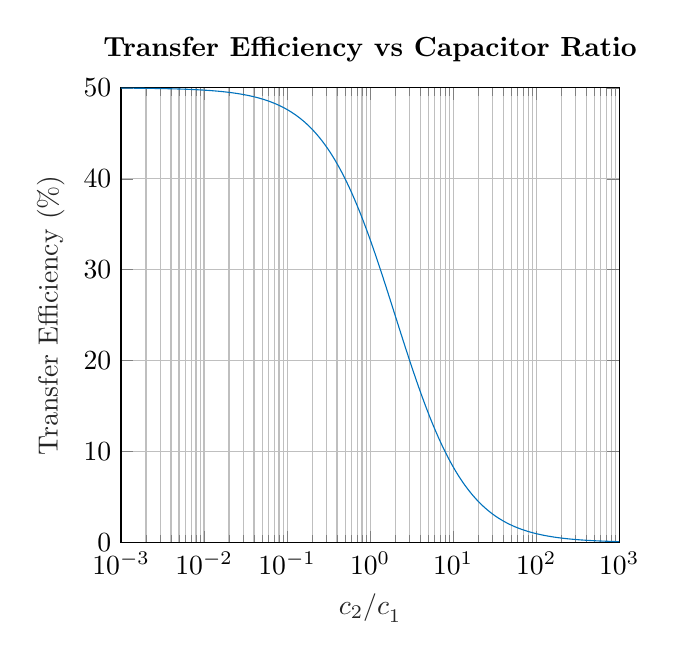
\begin{tikzpicture}

\begin{axis}[%
width=180pt,
height=164.293pt,
at={(0pt,0pt)},
scale only axis,
xmode=log,
xmin=0.001,
xmax=1000,
xminorticks=true,
xlabel style={font=\color{white!15!black}},
xlabel={$\text{c}_\text{2}\text{/c}_\text{1}$},
ymin=0,
ymax=50,
ylabel style={font=\color{white!15!black}},
ylabel={Transfer Efficiency (\%)},
axis background/.style={fill=white},
title style={font=\bfseries},
title={Transfer Efficiency vs Capacitor Ratio},
xmajorgrids,
xminorgrids,
ymajorgrids
]
\addplot [color=mycolor1, forget plot]
  table[row sep=crcr]{%
0.001	49.9750124937531\\
0.00101392540755882	49.9746647088587\\
0.00102804473209331	49.9743120858601\\
0.0010423606739764	49.9739545575231\\
0.0010568759711848	49.9735920556813\\
0.00107159339982267	49.973224511223\\
0.00108651577465254	49.9728518540781\\
0.00110164594963366	49.9724740132051\\
0.00111698681846782	49.9720909165775\\
0.00113254131515281	49.9717024911701\\
0.00114831241454351	49.9713086629457\\
0.00116430313292088	49.9709093568405\\
0.00118051652856881	49.9705044967503\\
0.00119695570235904	49.9700940055163\\
0.00121362379834424	49.9696778049102\\
0.00123052400435926	49.9692558156195\\
0.00124765955263087	49.9688279572327\\
0.0012650337203959	49.9683941482242\\
0.00128264983052806	49.9679543059388\\
0.00130051125217341	49.9675083465761\\
0.00131862140139475	49.9670561851748\\
0.00133698374182495	49.9665977355966\\
0.00135560178532937	49.9661329105103\\
0.00137447909267754	49.9656616213748\\
0.00139361927422414	49.9651837784231\\
0.00141302599059953	49.9646992906449\\
0.00143270295340983	49.9642080657697\\
0.00145265392594678	49.9637100102494\\
0.0014728827239075	49.9632050292407\\
0.00149339321612425	49.9626930265874\\
0.00151418932530435	49.9621739048022\\
0.00153527502878042	49.9616475650483\\
0.00155665435927106	49.9611139071212\\
0.00157833140565212	49.9605728294295\\
0.0016003103137387	49.9600242289759\\
0.00162259528707809	49.959468001338\\
0.00164519058775366	49.9589040406489\\
0.00166810053720006	49.9583322395768\\
0.00169132951702965	49.9577524893052\\
0.00171488196987054	49.9571646795126\\
0.00173876240021625	49.9565686983517\\
0.00176297537528721	49.9559644324285\\
0.00178752552590424	49.9553517667807\\
0.00181241754737424	49.9547305848568\\
0.00183765620038817	49.954100768494\\
0.00186324631193156	49.9534621978958\\
0.00188919277620767	49.95281475161\\
0.00191550055557353	49.9521583065059\\
0.00194217468148903	49.9514927377511\\
0.00196922025547917	49.9508179187883\\
0.00199664245010979	49.9501337213117\\
0.0020244465099768	49.9494400152429\\
0.00205263775270925	49.9487366687069\\
0.00208122156998634	49.9480235480068\\
0.0021102034285686	49.9473005176\\
0.00213958887134342	49.9465674400717\\
0.00216938351838518	49.9458241761101\\
0.00219959306803007	49.9450705844801\\
0.00223022329796594	49.9443065219969\\
0.00226128006633728	49.9435318434999\\
0.00229276931286565	49.9427464018248\\
0.00232469705998565	49.941950047777\\
0.00235706941399673	49.9411426301033\\
0.00238989256623105	49.940323995464\\
0.0024231727942376	49.9394939884047\\
0.00245691646298279	49.9386524513266\\
0.00249113002606779	49.9377992244581\\
0.00252582002696278	49.9369341458247\\
0.00256099310025846	49.9360570512189\\
0.00259665597293487	49.9351677741698\\
0.00263281546564802	49.9342661459126\\
0.00266947849403432	49.9333519953567\\
0.00270665207003324	49.9324251490543\\
0.00274434330322837	49.9314854311684\\
0.00278255940220713	49.9305326634401\\
0.00282130767593947	49.9295666651556\\
0.00286059553517574	49.9285872531131\\
0.00290043049386399	49.9275942415882\\
0.00294082017058706	49.9265874423005\\
0.00298177229001967	49.9255666643783\\
0.00302329468440578	49.9245317143233\\
0.00306539529505653	49.9234823959753\\
0.00310808217386906	49.9224185104756\\
0.00315136348486648	49.9213398562307\\
0.00319524750575921	49.9202462288751\\
0.0032397426295282	49.9191374212336\\
0.00328485736603004	49.918013223283\\
0.00333060034362459	49.9168734221138\\
0.00337698031082509	49.9157178018912\\
0.00342400613797143	49.9145461438148\\
0.00347168681892656	49.9133582260791\\
0.00352003147279668	49.9121538238325\\
0.00356904934567523	49.9109327091362\\
0.00361874981241128	49.9096946509222\\
0.00366914237840249	49.9084394149513\\
0.00372023668141307	49.90716676377\\
0.003772042493417	49.9058764566671\\
0.003824569722467	49.9045682496298\\
0.00387782841458946	49.9032418952991\\
0.00393182875570577	49.9018971429246\\
0.00398658107358044	49.9005337383186\\
0.00404209583979631	49.8991514238102\\
0.00409838367175726	49.8977499381979\\
0.00415545533471888	49.8963290167023\\
0.00421332174384729	49.8948883909178\\
0.00427199396630678	49.893427788764\\
0.0043314832233764	49.891946934436\\
0.00439180089259609	49.8904455483544\\
0.00445295850994266	49.8889233471148\\
0.0045149677720361	49.8873800434363\\
0.00457784053837662	49.8858153461093\\
0.00464158883361278	49.8842289599431\\
0.00470622484984128	49.8826205857122\\
0.00477176094893875	49.8809899201024\\
0.00483820966492596	49.8793366556563\\
0.00490558370636505	49.8776604807171\\
0.00497389595879006	49.8759610793733\\
0.00504315948717136	49.8742381314011\\
0.00511338753841433	49.8724913122072\\
0.00518459354389291	49.8707202927704\\
0.00525679112201842	49.8689247395822\\
0.00532999408084409	49.8671043145872\\
0.00540421642070592	49.8652586751226\\
0.00547947233690029	49.8633874738564\\
0.00555577622239888	49.8614903587258\\
0.00563314267060135	49.8595669728737\\
0.00571158647812644	49.8576169545853\\
0.00579112264764176	49.8556399372234\\
0.00587176639073326	49.8536355491633\\
0.00595353313081437	49.8516034137261\\
0.00603643850607586	49.8495431491122\\
0.0061204983724767	49.8474543683333\\
0.0062057288067765	49.8453366791434\\
0.00629214610961034	49.8431896839697\\
0.00637976680860628	49.8410129798419\\
0.00646860766154633	49.838806158321\\
0.00655868565957144	49.8365688054268\\
0.00665001803043112	49.8343005015653\\
0.00674262224177834	49.8320008214545\\
0.00683651600451024	49.8296693340492\\
0.00693171727615541	49.8273056024656\\
0.00702824426430835	49.8249091839043\\
0.00712611543011175	49.8224796295726\\
0.00722534949178721	49.8200164846061\\
0.00732596542821523	49.8175192879884\\
0.00742798248256492	49.8149875724712\\
0.00753142016597438	49.8124208644926\\
0.00763629826128224	49.8098186840939\\
0.00774263682681127	49.807180544837\\
0.00785045620020451	49.8045059537188\\
0.00795977700231499	49.8017944110863\\
0.00807062014114951	49.7990454105498\\
0.00818300681586739	49.7962584388949\\
0.00829695852083491	49.7934329759941\\
0.00841249704973612	49.7905684947168\\
0.00852964449974103	49.7876644608383\\
0.00864842327573173	49.7847203329484\\
0.00876885609458743	49.7817355623574\\
0.00889096598952916	49.778709593003\\
0.00901477631452492	49.775641861354\\
0.00914031074875623	49.7725317963147\\
0.00926759330114688	49.7693788191268\\
0.00939664831495469	49.7661823432712\\
0.00952750047242729	49.7629417743677\\
0.00966017479952265	49.7596565100742\\
0.0097946966706954	49.7563259399848\\
0.0099310918137498	49.7529494455258\\
0.0100693863147603	49.7495263998518\\
0.0102096066230605	49.7460561677394\\
0.0103517795563018	49.7425381054806\\
0.0104959323055823	49.7389715607744\\
0.0106420924406472	49.7353558726176\\
0.0107902879151618	49.7316903711936\\
0.0109405470720574	49.727974377761\\
0.0110928986489522	49.7242072045403\\
0.0112473717836475	49.720388154599\\
0.0114039960197003	49.7165165217364\\
0.0115628013120738	49.7125915903662\\
0.011723818032866	49.7086126353982\\
0.011887076977119	49.7045789221187\\
0.0120526093687084	49.7004897060696\\
0.0122204468663149	49.6963442329257\\
0.0123906215694792	49.6921417383715\\
0.0125631660247412	49.6878814479757\\
0.0127381132318648	49.6835625770654\\
0.0129154966501488	49.679184330598\\
0.0130953502048267	49.674745903032\\
0.0132777082935543	49.6702464781968\\
0.0134626057929891	49.6656852291606\\
0.0136500780654601	49.6610613180972\\
0.0138401609657313	49.6563738961514\\
0.0140328908478587	49.6516221033026\\
0.0142283045721435	49.6468050682277\\
0.0144264395121816	49.6419219081617\\
0.0146273335620113	49.6369717287577\\
0.014831025143361	49.6319536239446\\
0.0150375532129974	49.6268666757843\\
0.0152469572701757	49.6217099543267\\
0.0154592773641948	49.6164825174634\\
0.015674554102056	49.6111834107803\\
0.0158928286562298	49.6058116674083\\
0.0161141427725302	49.6003663078726\\
0.0163385387780986	49.5948463399405\\
0.0165660595894991	49.5892507584683\\
0.0167967487209265	49.5835785452456\\
0.0170306502925284	49.5778286688391\\
0.0172678090388436	49.5720000844342\\
0.0175082703173572	49.5660917336759\\
0.0177520801171764	49.5601025445072\\
0.0179992850678248	49.5540314310067\\
0.0182499324481615	49.5478772932244\\
0.018504070195423	49.5416390170164\\
0.0187617469143912	49.5353154738773\\
0.0190230118866894	49.5289055207718\\
0.0192879150802078	49.5224079999646\\
0.0195565071586595	49.5158217388487\\
0.0198288394912707	49.5091455497718\\
0.020104964162605	49.5023782298625\\
0.0203849339825246	49.4955185608531\\
0.0206688024962908	49.4885653089027\\
0.0209566239948043	49.4815172244177\\
0.0212484535249888	49.4743730418709\\
0.0215443469003188	49.4671314796197\\
0.0218443607114943	49.4597912397222\\
0.0221485523372636	49.452351007752\\
0.0224569799553977	49.4448094526121\\
0.0227697025538168	49.4371652263461\\
0.0230867799418717	49.4294169639491\\
0.0234082727617829	49.4215632831768\\
0.0237342425002387	49.4136027843528\\
0.0240647515001542	49.4055340501751\\
0.0243998629725955	49.3973556455204\\
0.0247396410088681	49.389066117248\\
0.0250841505927754	49.3806639940016\\
0.0254334576130465	49.3721477860097\\
0.025787628875938	49.3635159848852\\
0.0261467321180109	49.3547670634229\\
0.0265108360190854	49.3458994753967\\
0.0268800102153761	49.3369116553545\\
0.0272543253128103	49.3278020184122\\
0.0276338529005317	49.3185689600467\\
0.028018665564592	49.3092108558875\\
0.028408836901833	49.2997260615068\\
0.028804441533963	49.2901129122089\\
0.0292055551218275	49.2803697228181\\
0.0296122543798803	49.2704947874655\\
0.0300246170908555	49.260486379375\\
0.030442722120643	49.2503427506478\\
0.0308666494333727	49.2400621320463\\
0.0312964801067075	49.2296427327767\\
0.0317322963473498	49.2190827402705\\
0.0321741815067637	49.2083803199658\\
0.0326222200971167	49.1975336150867\\
0.0330764978074424	49.1865407464226\\
0.0335371015200293	49.1753998121067\\
0.0340041193270371	49.1641088873928\\
0.0344776405473446	49.152666024433\\
0.0349577557436328	49.1410692520529\\
0.0354445567397043	49.1293165755279\\
0.0359381366380463	49.1174059763576\\
0.0364385898376354	49.1053354120406\\
0.036946012051993	49.093102815848\\
0.0374605003274899	49.0807060965975\\
0.0379821530619073	49.0681431384264\\
0.0385110700232557	49.0554118005644\\
0.0390473523688556	49.0425099171068\\
0.0395911026646846	49.0294352967867\\
0.0401424249049932	49.0161857227477\\
0.0407014245321944	49.0027589523165\\
0.0412682084570295	48.9891527167754\\
0.0418428850790158	48.9753647211353\\
0.0424255643071778	48.9613926439084\\
0.0430163575810679	48.9472341368818\\
0.04361537789208	48.932886824891\\
0.044222739805059	48.9183483055942\\
0.0448385594802119	48.9036161492473\\
0.045462954695324	48.8886878984788\\
0.0460960448682843	48.8735610680668\\
0.0467379510799246	48.8582331447154\\
0.0473887960971765	48.8427015868332\\
0.0480487043965513	48.8269638243123\\
0.0487178021879463	48.8110172583086\\
0.0493962174387832	48.7948592610238\\
0.0500840798984821	48.7784871754879\\
0.0507815211232767	48.7618983153441\\
0.051488674501375	48.7450899646353\\
0.0522056752784698	48.7280593775917\\
0.0529326605836056	48.7108037784211\\
0.0536697694554048	48.6933203611008\\
0.0544171428686589	48.6756062891718\\
0.0551749237612913	48.6576586955354\\
0.0559432570616938	48.6394746822525\\
0.0567222897164454	48.6210513203446\\
0.0575121707184161	48.602385649599\\
0.0583130511352622	48.5834746783756\\
0.0591250841383188	48.5643153834178\\
0.0599484250318941	48.5449047096661\\
0.0607832312829723	48.5252395700752\\
0.0616296625513294	48.5053168454352\\
0.0624878807200689	48.4851333841959\\
0.0633580499265825	48.4646860022952\\
0.0642403365939419	48.4439714829926\\
0.065134909462728	48.4229865767057\\
0.0660419396233031	48.4017280008521\\
0.0669616005485322	48.380192439696\\
0.0678940681269611	48.3583765441995\\
0.068839520696455	48.3362769318792\\
0.0697981390783066	48.3138901866684\\
0.0707701066118189	48.2912128587849\\
0.0717556091893692	48.2682414646039\\
0.0727548352919623	48.2449724865383\\
0.0737679760252773	48.2214023729244\\
0.0747952251562182	48.1975275379143\\
0.0758367791499719	48.1733443613754\\
0.0768928372075831	48.1488491887967\\
0.0779636013040523	48.1240383312026\\
0.0790492762269642	48.0989080650743\\
0.080150069615654	48.0734546322789\\
0.0812661920009195	48.047674240007\\
0.0823978568452852	48.021563060718\\
0.0835452805838287	47.9951172320954\\
0.0847086826655741	47.9683328570095\\
0.0858882855954625	47.9412060034906\\
0.0870843149769072	47.9137327047118\\
0.0882969995549409	47.8859089589805\\
0.089526571259964	47.8577307297418\\
0.0907732652521023	47.8291939455913\\
0.0920373199661822	47.8002945002991\\
0.0933189771573324	47.7710282528452\\
0.09461848194722	47.7413910274663\\
0.0959360828709314	47.7113786137142\\
0.0972720319245054	47.6809867665272\\
0.0986265846131282	47.6502112063135\\
0.1	47.6190476190476\\
0.101392540755882	47.5874916563801\\
0.102804473209331	47.5555389357616\\
0.10423606739764	47.5231850405798\\
0.10568759711848	47.490425520312\\
0.107159339982267	47.457255890692\\
0.108651577465254	47.4236716338917\\
0.110164594963366	47.3896681987199\\
0.111698681846782	47.355241000835\\
0.113254131515281	47.3203854229762\\
0.114831241454351	47.2850968152101\\
0.116430313292088	47.2493704951953\\
0.118051652856881	47.2132017484642\\
0.119695570235904	47.1765858287239\\
0.121362379834424	47.1395179581742\\
0.123052400435926	47.1019933278458\\
0.124765955263087	47.0640070979573\\
0.12650337203959	47.0255543982924\\
0.128264983052806	46.986630328597\\
0.130051125217341	46.9472299589976\\
0.131862140139475	46.9073483304402\\
0.133698374182495	46.8669804551517\\
0.135560178532937	46.8261213171229\\
0.137447909267754	46.7847658726139\\
0.139361927422414	46.7429090506831\\
0.141302599059953	46.7005457537392\\
0.143270295340983	46.6576708581176\\
0.145265392594678	46.6142792146807\\
0.14728827239075	46.5703656494439\\
0.149339321612425	46.5259249642259\\
0.151418932530435	46.4809519373258\\
0.153527502878042	46.4354413242259\\
0.155665435927106	46.3893878583214\\
0.157833140565212	46.3427862516777\\
0.16003103137387	46.2956311958147\\
0.162259528707809	46.2479173625199\\
0.164519058775366	46.1996394046896\\
0.166810053720006	46.1507919571994\\
0.169132951702965	46.1013696378043\\
0.171488196987054	46.0513670480688\\
0.173876240021625	46.0007787743267\\
0.176297537528721	45.9495993886729\\
0.178752552590424	45.8978234499853\\
0.181241754737424	45.8454455049793\\
0.183765620038817	45.792460089294\\
0.186324631193156	45.7388617286109\\
0.188919277620767	45.6846449398054\\
0.191550055557353	45.629804232132\\
0.194217468148903	45.574334108443\\
0.196922025547917	45.5182290664412\\
0.199664245010979	45.4614835999668\\
0.20244465099768	45.4040922003199\\
0.205263775270925	45.3460493576169\\
0.208122156998634	45.2873495621836\\
0.211020342856859	45.2279873059829\\
0.213958887134342	45.1679570840793\\
0.216938351838518	45.1072533961395\\
0.219959306803007	45.0458707479694\\
0.223022329796594	44.9838036530879\\
0.226128006633728	44.9210466343382\\
0.229276931286565	44.8575942255356\\
0.232469705998565	44.7934409731535\\
0.235706941399673	44.728581438046\\
0.238989256623105	44.6630101972094\\
0.24231727942376	44.5967218455804\\
0.245691646298279	44.529710997873\\
0.249113002606779	44.4619722904529\\
0.252582002696278	44.3935003832503\\
0.256099310025846	44.3242899617102\\
0.259665597293487	44.2543357387814\\
0.263281546564802	44.1836324569427\\
0.266947849403432	44.1121748902675\\
0.270665207003324	44.0399578465262\\
0.274434330322837	43.9669761693255\\
0.278255940220713	43.8932247402863\\
0.282130767593947	43.8186984812575\\
0.286059553517574	43.743392356568\\
0.290043049386399	43.6673013753145\\
0.294082017058706	43.5904205936858\\
0.298177229001967	43.5127451173238\\
0.302329468440578	43.4342701037191\\
0.306539529505653	43.3549907646423\\
0.310808217386906	43.27490236861\\
0.315136348486648	43.1940002433842\\
0.319524750575921	43.1122797785067\\
0.32397426295282	43.0297364278643\\
0.328485736603004	42.9463657122885\\
0.333060034362459	42.8621632221849\\
0.337698031082509	42.7771246201946\\
0.342400613797143	42.6912456438847\\
0.347168681892656	42.6045221084683\\
0.352003147279668	42.5169499095527\\
0.356904934567523	42.4285250259147\\
0.361874981241128	42.3392435223018\\
0.366914237840249	42.2491015522588\\
0.372023668141307	42.1580953609788\\
0.3772042493417	42.0662212881759\\
0.3824569722467	41.9734757709803\\
0.387782841458946	41.8798553468537\\
0.393182875570577	41.785356656523\\
0.398658107358044	41.6899764469323\\
0.404209583979631	41.5937115742099\\
0.409838367175726	41.4965590066514\\
0.415545533471888	41.3985158277141\\
0.421332174384729	41.2995792390238\\
0.427199396630678	41.1997465633912\\
0.43314832233764	41.0990152478355\\
0.439180089259609	40.9973828666149\\
0.445295850994266	40.8948471242609\\
0.45149677720361	40.7914058586153\\
0.457784053837662	40.6870570438671\\
0.464158883361278	40.5817987935881\\
0.470622484984128	40.4756293637643\\
0.477176094893875	40.3685471558227\\
0.483820966492596	40.2605507196479\\
0.490558370636505	40.1516387565907\\
0.497389595879006	40.0418101224623\\
0.504315948717136	39.9310638305147\\
0.511338753841433	39.8193990544033\\
0.518459354389291	39.7068151311298\\
0.525679112201842	39.5933115639626\\
0.532999408084409	39.4788880253333\\
0.540421642070592	39.3635443597049\\
0.547947233690029	39.2472805864101\\
0.555577622239888	39.130096902458\\
0.563314267060136	39.0119936853041\\
0.571158647812643	38.8929714955834\\
0.579112264764176	38.773031079802\\
0.587176639073326	38.6521733729855\\
0.595353313081437	38.5303995012806\\
0.603643850607587	38.4077107845084\\
0.61204983724767	38.2841087386642\\
0.62057288067765	38.1595950783636\\
0.629214610961034	38.0341717192298\\
0.637976680860628	37.9078407802208\\
0.646860766154633	37.7806045858922\\
0.655868565957143	37.6524656685943\\
0.665001803043112	37.5234267705981\\
0.674262224177834	37.3934908461505\\
0.683651600451024	37.2626610634531\\
0.693171727615541	37.1309408065624\\
0.702824426430835	36.9983336772094\\
0.712611543011175	36.8648434965345\\
0.722534949178721	36.7304743067361\\
0.732596542821523	36.5952303726278\\
0.742798248256492	36.4591161831049\\
0.753142016597438	36.3221364525134\\
0.763629826128224	36.1842961219222\\
0.774263682681127	36.0456003602935\\
0.785045620020451	35.9060545655499\\
0.795977700231499	35.7656643655349\\
0.807062014114951	35.6244356188651\\
0.818300681586739	35.4823744156705\\
0.829695852083491	35.339487078221\\
0.841249704973612	35.1957801614374\\
0.852964449974102	35.0512604532831\\
0.864842327573173	34.905934975036\\
0.876885609458743	34.7598109814363\\
0.889096598952916	34.6128959607106\\
0.901477631452492	34.4651976344686\\
0.914031074875623	34.3167239574712\\
0.926759330114688	34.1674831172679\\
0.939664831495469	34.017483533702\\
0.952750047242729	33.8667338582823\\
0.966017479952265	33.7152429734195\\
0.97946966706954	33.5630199915259\\
0.99310918137498	33.4100742539775\\
1.00693863147603	33.2564153299373\\
1.02096066230605	33.1020530150383\\
1.03517795563018	32.9469973299268\\
1.04959323055823	32.7912585186632\\
1.06420924406472	32.6348470469818\\
1.07902879151618	32.4777736004079\\
1.09405470720574	32.3200490822318\\
1.10928986489522	32.1616846113413\\
1.12473717836475	32.0026915199096\\
1.14039960197003	31.8430813509428\\
1.15628013120738	31.6828658556827\\
1.1723818032866	31.5220569908703\\
1.1887076977119	31.3606669158657\\
1.20526093687084	31.1987079896296\\
1.22204468663149	31.0361927675639\\
1.23906215694792	30.8731339982149\\
1.25631660247412	30.7095446198385\\
1.27381132318648	30.5454377568307\\
1.29154966501488	30.3808267160228\\
1.30953502048267	30.2157249828454\\
1.32777082935543	30.0501462173612\\
1.34626057929891	29.8841042501691\\
1.36500780654601	29.7176130781831\\
1.38401609657313	29.550686860286\\
1.40328908478587	29.3833399128631\\
1.42283045721435	29.215586705216\\
1.44264395121816	29.0474418548615\\
1.46273335620113	28.8789201227169\\
1.4831025143361	28.7100364081763\\
1.50375532129974	28.5408057440793\\
1.52469572701757	28.3712432915777\\
1.54592773641948	28.201364334902\\
1.5674554102056	28.0311842760319\\
1.58928286562298	27.8607186292751\\
1.61141427725302	27.6899830157574\\
1.63385387780986	27.518993157829\\
1.65660595894991	27.3477648733903\\
1.67967487209265	27.1763140701421\\
1.70306502925284	27.0046567397648\\
1.72678090388436	26.8328089520293\\
1.75082703173573	26.6607868488471\\
1.77520801171763	26.488606638261\\
1.79992850678248	26.3162845883838\\
1.82499324481615	26.1438370212877\\
1.8504070195423	25.971280306851\\
1.87617469143912	25.7986308565656\\
1.90230118866894	25.6259051173109\\
1.92879150802078	25.4531195650994\\
1.95565071586595	25.2802906987981\\
1.98288394912707	25.107435033832\\
2.0104964162605	24.9345690958734\\
2.03849339825246	24.7617094145238\\
2.06688024962908	24.5888725169915\\
2.09566239948043	24.4160749217723\\
2.12484535249888	24.2433331323364\\
2.15443469003188	24.0706636308278\\
2.18443607114943	23.8980828717813\\
2.21485523372636	23.7256072758613\\
2.24569799553977	23.5532532236284\\
2.27697025538168	23.381037049339\\
2.30867799418717	23.2089750347809\\
2.34082727617829	23.0370834031528\\
2.37342425002387	22.8653783129899\\
2.40647515001542	22.6938758521423\\
2.43998629725955	22.5225920318092\\
2.47396410088681	22.3515427806357\\
2.50841505927754	22.1807439388743\\
2.54334576130465	22.0102112526176\\
2.5787628875938	21.8399603681053\\
2.61467321180109	21.6700068261107\\
2.65108360190854	21.5003660564101\\
2.68800102153761	21.3310533723393\\
2.72543253128103	21.1620839654419\\
2.76338529005317	20.9934729002121\\
2.8018665564592	20.8252351089361\\
2.8408836901833	20.6573853866366\\
2.8804441533963	20.4899383861221\\
2.92055551218275	20.3229086131456\\
2.96122543798803	20.1563104216755\\
3.00246170908555	19.9901580092814\\
3.0442722120643	19.8244654126381\\
3.08666494333727	19.6592465031502\\
3.12964801067075	19.4945149827004\\
3.17322963473498	19.3302843795224\\
3.21741815067637	19.1665680442033\\
3.26222200971167	19.0033791458143\\
3.30764978074424	18.8407306681749\\
3.35371015200293	18.6786354062496\\
3.40041193270371	18.5171059626807\\
3.44776405473446	18.3561547444577\\
3.49577557436328	18.1957939597244\\
3.54445567397044	18.0360356147259\\
3.59381366380463	17.8768915108955\\
3.64385898376354	17.718373242082\\
3.6946012051993	17.5604921919199\\
3.74605003274899	17.4032595313408\\
3.79821530619074	17.2466862162277\\
3.85110700232557	17.0907829852119\\
3.90473523688556	16.935560357613\\
3.95911026646846	16.7810286315213\\
4.01424249049932	16.6271978820225\\
4.07014245321944	16.4740779595646\\
4.12682084570295	16.3216784884668\\
4.18428850790158	16.1700088655682\\
4.24255643071778	16.0190782590173\\
4.3016357581068	15.8688956072007\\
4.36153778920801	15.7194696178091\\
4.4222739805059	15.5708087670409\\
4.48385594802119	15.4229212989408\\
4.5462954695324	15.275815224873\\
4.60960448682843	15.1294983231265\\
4.67379510799246	14.9839781386517\\
4.73887960971766	14.8392619829262\\
4.80487043965513	14.6953569339474\\
4.87178021879463	14.5522698363512\\
4.93962174387832	14.4100073016535\\
5.00840798984821	14.2685757086134\\
5.07815211232768	14.1279812037149\\
5.14886745013749	13.9882297017658\\
5.22056752784698	13.8493268866108\\
5.29326605836056	13.7112782119564\\
5.36697694554048	13.5740889023053\\
5.44171428686589	13.4377639539982\\
5.51749237612912	13.3023081363591\\
5.59432570616938	13.1677259929428\\
5.67222897164454	13.0340218428811\\
5.75121707184161	12.9011997823254\\
5.83130511352622	12.7692636859826\\
5.91250841383188	12.6382172087413\\
5.99484250318941	12.5080637873863\\
6.07832312829723	12.3788066423976\\
6.16296625513294	12.2504487798316\\
6.24878807200689	12.1229929932811\\
6.33580499265825	11.9964418659116\\
6.42403365939419	11.870797772571\\
6.5134909462728	11.7460628819697\\
6.6041939623303	11.6222391589272\\
6.69616005485322	11.4993283666842\\
6.78940681269611	11.377332069276\\
6.8839520696455	11.2562516339634\\
6.97981390783066	11.1360882337213\\
7.07701066118189	11.016842849778\\
7.17556091893693	10.8985162742057\\
7.27548352919623	10.7811091125581\\
7.37679760252773	10.6646217865514\\
7.47952251562182	10.5490545367875\\
7.58367791499719	10.434407425516\\
7.68928372075831	10.3206803394311\\
7.79636013040524	10.2078729925033\\
7.90492762269642	10.0959849288406\\
8.0150069615654	9.98501552557777\\
8.12661920009194	9.87496399579161\\
8.23978568452852	9.76582939143852\\
8.35452805838287	9.65761060631262\\
8.4708682665574	9.55030637902179\\
8.58882855954625	9.44391529597918\\
8.70843149769072	9.3384357944079\\
8.82969995549409	9.23386616535653\\
8.9526571259964	9.13020455672327\\
9.07732652521022	9.02744897628647\\
9.20373199661822	8.92559729473932\\
9.33189771573324	8.8246472487269\\
9.461848194722	8.72459644388314\\
9.59360828709315	8.62544235786604\\
9.72720319245054	8.52718234338906\\
9.86265846131282	8.4298136312468\\
10	8.33333333333333\\
10.1392540755881	8.23773844565116\\
10.2804473209331	8.14302585130928\\
10.423606739764	8.04919232350875\\
10.5687597118481	7.95623452851391\\
10.7159339982267	7.86414902860816\\
10.8651577465254	7.77293228503226\\
11.0164594963366	7.68258066090434\\
11.1698681846782	7.59309042411978\\
11.3254131515281	7.50445775022985\\
11.4831241454351	7.41667872529797\\
11.6430313292088	7.32974934873214\\
11.8051652856881	7.24366553609256\\
11.9695570235904	7.1584231218735\\
12.1362379834424	7.07401786225788\\
12.3052400435926	6.99044543784433\\
12.4765955263087	6.907701456345\\
12.650337203959	6.82578145525391\\
12.8264983052806	6.74468090448465\\
13.0051125217341	6.66439520897663\\
13.1862140139475	6.58491971126951\\
13.3698374182495	6.50624969404455\\
13.5560178532937	6.42838038263288\\
13.7447909267754	6.35130694748963\\
13.9361927422414	6.27502450663351\\
14.1302599059953	6.19952812805154\\
14.3270295340983	6.12481283206809\\
14.5265392594678	6.05087359367821\\
14.728827239075	5.97770534484456\\
14.9339321612425	5.90530297675779\\
15.1418932530435	5.83366134206005\\
15.3527502878042	5.76277525703125\\
15.5665435927106	5.69263950373799\\
15.7833140565212	5.62324883214498\\
16.003103137387	5.55459796218854\\
16.2259528707809	5.48668158581251\\
16.4519058775366	5.41949436896598\\
16.6810053720006	5.35303095356322\\
16.9132951702965	5.28728595940548\\
17.1488196987054	5.22225398606477\\
17.3876240021625	5.15792961472979\\
17.629753752872	5.09430741001369\\
17.8752552590424	5.03138192172422\\
18.1241754737424	4.96914768659606\\
18.3765620038817	4.90759922998542\\
18.6324631193156	4.84673106752739\\
18.8919277620767	4.78653770675588\\
19.1550055557353	4.72701364868653\\
19.4217468148902	4.66815338936272\\
19.6922025547917	4.60995142136502\\
19.9664245010979	4.55240223528421\\
20.2444650997681	4.49550032115821\\
20.5263775270925	4.43924016987329\\
20.8122156998634	4.38361627452957\\
21.102034285686	4.32862313177156\\
21.3958887134342	4.27425524308375\\
21.6938351838519	4.22050711605158\\
21.9959306803007	4.16737326558849\\
22.3022329796594	4.11484821512898\\
22.6128006633728	4.06292649778835\\
22.9276931286565	4.01160265748945\\
23.2469705998565	3.96087125005676\\
23.5706941399673	3.91072684427831\\
23.8989256623105	3.86116402293572\\
24.231727942376	3.81217738380304\\
24.5691646298279	3.76376154061445\\
24.9113002606779	3.71591112400159\\
25.2582002696278	3.66862078240081\\
25.6099310025846	3.6218851829307\\
25.9665597293487	3.5756990122406\\
26.3281546564802	3.53005697733031\\
26.6947849403432	3.4849538063415\\
27.0665207003324	3.44038424932147\\
27.4434330322836	3.39634307895936\\
27.8255940220713	3.35282509129571\\
28.2130767593947	3.30982510640546\\
28.6059553517574	3.26733796905503\\
29.0043049386399	3.22535854933398\\
29.4082017058706	3.18388174326162\\
29.8177229001967	3.14290247336907\\
30.2329468440578	3.10241568925726\\
30.6539529505653	3.06241636813128\\
31.0808217386906	3.02289951531168\\
31.5136348486648	2.9838601647229\\
31.9524750575921	2.94529337935966\\
32.397426295282	2.90719425173145\\
32.8485736603005	2.86955790428577\\
33.3060034362459	2.83237948981045\\
33.7698031082509	2.79565419181559\\
34.2400613797143	2.75937722489554\\
34.7168681892656	2.7235438350713\\
35.2003147279668	2.68814930011388\\
35.6904934567523	2.65318892984896\\
36.1874981241128	2.6186580664434\\
36.6914237840249	2.58455208467382\\
37.2023668141307	2.550866392178\\
37.72042493417	2.51759642968909\\
38.24569722467	2.4847376712535\\
38.7782841458945	2.45228562443248\\
39.3182875570577	2.42023583048806\\
39.8658107358044	2.38858386455367\\
40.4209583979631	2.35732533578972\\
40.9838367175726	2.32645588752477\\
41.5545533471887	2.29597119738239\\
42.1332174384729	2.26586697739435\\
42.7199396630678	2.23613897410031\\
43.314832233764	2.2067829686345\\
43.9180089259609	2.17779477679971\\
44.5295850994265	2.14917024912893\\
45.149677720361	2.120905270935\\
45.7784053837662	2.09299576234868\\
46.4158883361278	2.06543767834536\\
47.0622484984128	2.03822700876082\\
47.7176094893874	2.01135977829637\\
48.3820966492596	1.98483204651368\\
49.0558370636505	1.95863990781958\\
49.7389595879007	1.93277949144121\\
50.4315948717136	1.90724696139177\\
51.1338753841432	1.88203851642719\\
51.8459354389291	1.85715038999402\\
52.5679112201842	1.83257885016883\\
53.2999408084409	1.80832019958937\\
54.0421642070592	1.7843707753778\\
54.7947233690028	1.76072694905628\\
55.5577622239888	1.73738512645515\\
56.3314267060135	1.71434174761391\\
57.1158647812643	1.69159328667544\\
57.9112264764176	1.66913625177348\\
58.7176639073326	1.64696718491377\\
59.5353313081437	1.62508266184903\\
60.3643850607586	1.60347929194804\\
61.204983724767	1.58215371805902\\
62.057288067765	1.56110261636758\\
62.9214610961035	1.54032269624939\\
63.7976680860628	1.51981070011783\\
64.6860766154632	1.49956340326688\\
65.5868565957144	1.4795776137093\\
66.5001803043112	1.45985017201052\\
67.4262224177835	1.44037795111815\\
68.3651600451024	1.42115785618767\\
69.317172761554	1.40218682440407\\
70.2824426430835	1.38346182479998\\
71.2611543011175	1.36497985807022\\
72.2534949178722	1.34673795638313\\
73.2596542821523	1.32873318318863\\
74.2798248256491	1.31096263302344\\
75.3142016597438	1.29342343131337\\
76.3629826128224	1.276112734173\\
77.4263682681128	1.25902772820279\\
78.5045620020451	1.2421656302839\\
79.5977700231498	1.22552368737074\\
80.7062014114951	1.20909917628137\\
81.8300681586739	1.1928894034861\\
82.9695852083491	1.17689170489412\\
84.1249704973612	1.1611034456385\\
85.2964449974102	1.14552201985965\\
86.4842327573173	1.13014485048728\\
87.6885609458743	1.11496938902107\\
88.9096598952917	1.09999311531006\\
90.1477631452492	1.08521353733105\\
91.4031074875622	1.07062819096588\\
92.6759330114688	1.05623463977784\\
93.9664831495469	1.04203047478741\\
95.275004724273	1.02801331424708\\
96.6017479952265	1.01418080341579\\
97.9469667069539	1.00053061433272\\
99.310918137498	0.987060445590683\\
100.693863147603	0.973768022109259\\
102.096066230605	0.960651094907557\\
103.517795563018	0.947707440876906\\
104.959323055823	0.934934862553398\\
106.420924406472	0.922331187890428\\
107.902879151618	0.9098942700313\\
109.405470720574	0.897621987081933\\
110.928986489522	0.88551224188378\\
112.473717836475	0.873562961786996\\
114.039960197003	0.861772098423923\\
115.628013120738	0.850137627482974\\
117.23818032866	0.838657548482934\\
118.87076977119	0.827329884547778\\
120.526093687084	0.816152682182027\\
122.204468663149	0.805124011046711\\
123.906215694792	0.794241963736003\\
125.631660247412	0.783504655554519\\
127.381132318648	0.772910224295408\\
129.154966501488	0.762456830019207\\
130.953502048267	0.752142654833541\\
132.777082935543	0.741965902673713\\
134.626057929891	0.731924799084187\\
136.500780654601	0.722017591001049\\
138.401609657313	0.712242546535444\\
140.328908478587	0.702597954758042\\
142.283045721435	0.693082125484572\\
144.264395121816	0.683693389062426\\
146.273335620113	0.674430096158403\\
148.31025143361	0.665290617547589\\
150.375532129974	0.656273343903414\\
152.469572701757	0.647376685588918\\
154.592773641948	0.638599072449229\\
156.74554102056	0.629938953605309\\
158.928286562298	0.621394797248951\\
161.141427725302	0.612965090439078\\
163.385387780986	0.604648338899362\\
165.660595894992	0.596443066817152\\
167.967487209265	0.588347816643775\\
170.306502925284	0.580361148896174\\
172.678090388436	0.572481641959949\\
175.082703173572	0.56470789189378\\
177.520801171764	0.557038512235254\\
179.992850678248	0.549472133808124\\
182.499324481615	0.542007404530983\\
185.04070195423	0.534642989227396\\
187.617469143912	0.527377569437466\\
190.230118866895	0.520209843230877\\
192.879150802078	0.513138525021394\\
195.565071586595	0.506162345382842\\
198.288394912707	0.49928005086657\\
201.04964162605	0.492490403820396\\
203.849339825246	0.485792182209056\\
206.688024962908	0.479184179436141\\
209.566239948044	0.472665204167536\\
212.484535249888	0.466234080156378\\
215.443469003188	0.459889646069498\\
218.443607114943	0.453630755315387\\
221.485523372636	0.44745627587368\\
224.569799553978	0.441365090126128\\
227.697025538168	0.435356094689103\\
230.867799418717	0.429428200247606\\
234.082727617829	0.423580331390782\\
237.342425002387	0.417811426448958\\
240.647515001543	0.41212043733217\\
243.998629725955	0.406506329370212\\
247.396410088681	0.400968081154182\\
250.841505927754	0.395504684379524\\
254.334576130465	0.390115143690579\\
257.87628875938	0.384798476526614\\
261.467321180109	0.379553712969355\\
265.108360190854	0.374379895591992\\
268.800102153761	0.369276079309674\\
272.543253128103	0.364241331231475\\
276.338529005317	0.359274730513826\\
280.18665564592	0.354375368215418\\
284.08836901833	0.349542347153557\\
288.04441533963	0.344774781761973\\
292.055551218275	0.340071797950078\\
296.122543798804	0.335432532963652\\
300.246170908555	0.330856135246971\\
304.42722120643	0.326341764306355\\
308.666494333727	0.32188859057513\\
312.964801067075	0.317495795280006\\
317.322963473498	0.313162570308851\\
321.741815067637	0.308888118079858\\
326.222200971167	0.304671651412101\\
330.764978074424	0.300512393397464\\
335.371015200293	0.296409577273944\\
340.041193270371	0.292362446300302\\
344.776405473446	0.288370253632084\\
349.577557436327	0.284432262198962\\
354.445567397044	0.280547744583426\\
359.381366380463	0.276715982900789\\
364.385898376355	0.272936268680513\\
369.46012051993	0.269207902748835\\
374.605003274899	0.265530195112692\\
379.821530619074	0.261902464844932\\
385.110700232557	0.258324039970802\\
390.473523688556	0.254794257355699\\
395.911026646846	0.251312462594187\\
401.424249049932	0.24787800990025\\
407.014245321944	0.244490261998791\\
412.682084570295	0.241148590018358\\
418.428850790158	0.237852373385078\\
424.255643071778	0.234600999717817\\
430.163575810679	0.231393864724517\\
436.153778920801	0.228230372099737\\
442.22739805059	0.225109933423358\\
448.385594802119	0.22203196806047\\
454.62954695324	0.218995903062401\\
460.960448682843	0.216001173068904\\
467.379510799246	0.213047220211472\\
473.887960971765	0.210133494017793\\
480.487043965513	0.207259451317304\\
487.178021879463	0.204424556147865\\
493.962174387832	0.201628279663526\\
500.840798984821	0.198870100043371\\
507.815211232767	0.196149502401455\\
514.88674501375	0.19346597869779\\
522.056752784698	0.190819027650396\\
529.326605836056	0.188208154648397\\
536.697694554048	0.185632871666146\\
544.171428686589	0.183092697178386\\
551.749237612913	0.180587156076417\\
559.432570616938	0.178115779585274\\
567.222897164455	0.175678105181895\\
575.121707184161	0.173273676514285\\
583.130511352622	0.170902043321641\\
591.250841383188	0.16856276135546\\
599.484250318941	0.166255392301585\\
607.832312829724	0.163979503703212\\
616.296625513294	0.161734668884829\\
624.878807200689	0.159520466877079\\
633.580499265825	0.15733648234254\\
642.403365939419	0.155182305502422\\
651.349094627281	0.153057532064152\\
660.419396233031	0.150961763149854\\
669.616005485321	0.148894605225702\\
678.940681269611	0.146855670032154\\
688.39520696455	0.144844574515035\\
697.981390783067	0.142860940757483\\
707.701066118189	0.140904395912725\\
717.556091893692	0.138974572137698\\
727.548352919623	0.137071106527489\\
737.679760252773	0.13519364105059\\
747.952251562183	0.133341822484959\\
758.367791499719	0.131515302354883\\
768.928372075831	0.129713736868623\\
779.636013040524	0.127936786856846\\
790.492762269642	0.126184117711823\\
801.500696156541	0.124455399327392\\
812.661920009195	0.122750306039678\\
823.978568452851	0.121068516568549\\
835.452805838287	0.119409713959822\\
847.08682665574	0.117773585528191\\
858.882855954626	0.116159822800874\\
870.843149769072	0.11456812146198\\
882.969995549408	0.112998181297568\\
895.26571259964	0.111449706141418\\
907.732652521022	0.109922403821478\\
920.373199661823	0.108415986106994\\
933.189771573324	0.106930168656319\\
946.184819472199	0.105464670965376\\
959.360828709315	0.104019216316787\\
972.720319245054	0.102593531729648\\
986.265846131283	0.101187347909943\\
1000	0.0998003992015968\\
};
\end{axis}
\end{tikzpicture}%
    \caption{Efficiency of energy transfer for different $C_1$ to $C_2$ ratios.}
    \label{fig:transfer-efficiency}
\end{figure}

From  this  graph  we  see   that   for  $C_1=C_2$,  the  resistor  dissipates
\SI{33}{\percent} of the energy. As the  value  of  $C_2$  grows  larger  than
$C_1$, more and more energy is dissipated on $R$ versus being transferred into
$C_2$.

As the value of $C_2$ grows smaller  than $C_1$, the energy transfer gets more
and  more  efficient, peaking at a theoretical maximum  of  \SI{50}{\percent}.

